\subsection{FrontierMath}
{{\footnotesize
\noindent FrontierMath is a benchmark of hundreds of expert-vetted mathematics problems spanning
number theory, real analysis, algebraic geometry, and category theory, measuring LLMs 
ability to solve problems requiring deep abstract reasoning.


\begin{description}[labelwidth=4cm, labelsep=1em, leftmargin=4cm, itemsep=0.1em, parsep=0em]
  \item[date:] 2024-11-07
  \item[version:] 1
  \item[last\_updated:] 2024-11-07
  \item[expired:] false
  \item[valid:] yes
  \item[valid\_date:] 2024-11-07
  \item[url:] \href{https://arxiv.org/abs/2411.04872}{https://arxiv.org/abs/2411.04872}
  \item[doi:] 10.48550/arXiv.2411.04872
  \item[domain:] Mathematics
  \item[focus:] Challenging advanced mathematical reasoning
  \item[keywords:]
    - symbolic reasoning
    - number theory
    - algebraic geometry
    - category theory
  \item[licensing:] unknown
  \item[task\_types:]
    - Problem solving
  \item[ai\_capability\_measured:]
    - Symbolic and abstract mathematical reasoning
  \item[metrics:]
    - Accuracy
  \item[models:]
    - unkown
  \item[ml\_motif:]
    - Math problem solving
  \item[type:] Benchmark
  \item[ml\_task:]
    - Supervised Learning
  \item[solutions:] 0
  \item[notes:] Good
  \item[contact.name:] FrontierMath team
  \item[contact.email:] math\_evals@epochai.org
  \item[datasets.links.name:] unknown
  \item[datasets.links.url:] \href{unknown}{unknown}
  \item[results.links.name:] unknown
  \item[results.links.url:] \href{unknown}{unknown}
  \item[fair.reproducible:] True
  \item[fair.benchmark\_ready:] True
  \item[id:] frontiermath
  \item[Citations:] \cite{glazer2024frontiermathbenchmarkevaluatingadvanced}
\end{description}

{\bf Ratings:} ~ \\

\begin{tabular}{p{0.15\textwidth} p{0.07\textwidth} p{0.7\textwidth}}
\hline
Rating & Value & Reason \\
\hline
dataset & 0 & Paper and website had no link to any dataset. It may still exist somewhere
 \\
documentation & 0 & No specified way to reproduce the reference solution
 \\
metrics & 5 & (by default) All questions in the dataset have a correct answer
 \\
reference\_solution & 2 & Displays result of leading models on the benchmark, but none are trainable or list constraints
 \\
software & 0 & No link to code provided
 \\
specification & 3 & Well-specified process for asking questions and receiving answers. No software or hardware constraints
 \\
\hline
\end{tabular}

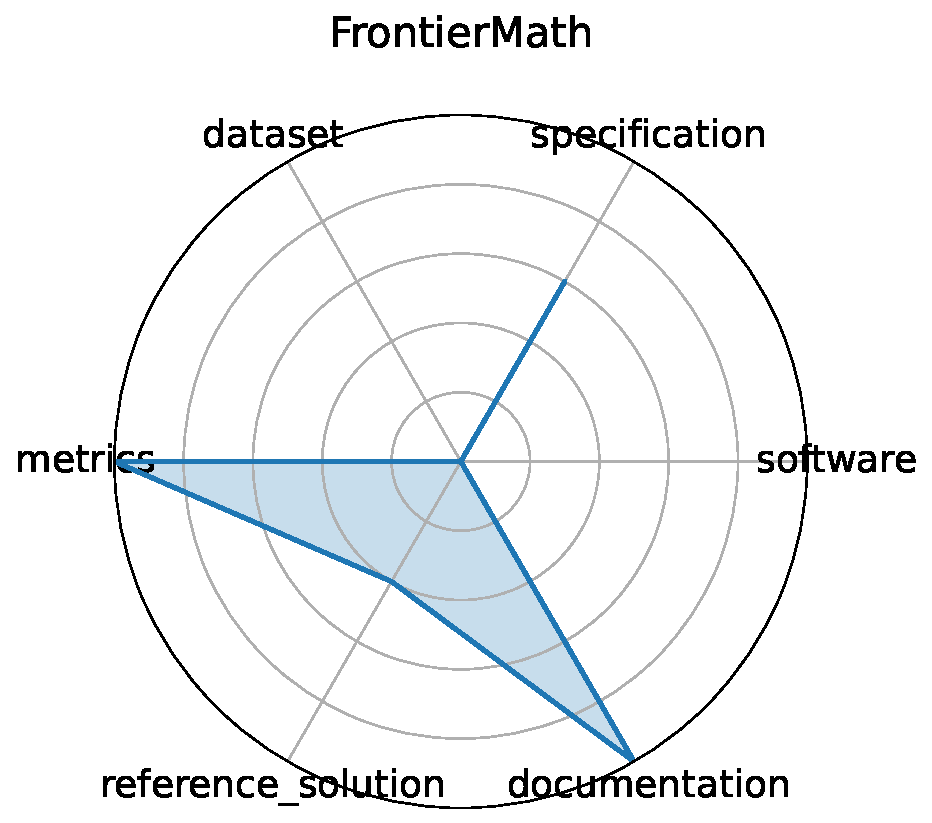
\includegraphics[width=0.2\textwidth]{frontiermath_radar.pdf}
}}
\clearpage